\documentclass[../main.tex]{subfiles}
\graphicspath{{\subfix{../figures/}}}
% \addbibresource{../bibliografia/bibliografia.bib}
% \addbibresource{../bibliografia/TFG.bib}
    
% \usepackage[showframe]{geometry}
% \usepackage{sidecap}
% \sidecaptionvpos{figure}{t}

\begin{document}

\chapter{Design of the Solution} \label{chap:solution_design}
    % \section{Technical Approach} \label{technical_approach}
        %% recuerda aqui incluir un resumen de la seccion al igual que en las otras , explicando que vas a tratar
    
    The work in this thesis is driven by the problem of designing an end-to-end platform that can be used to continuously develop ML models to aid in the research of TB while taking full advantage of the techniques we've discussed in the previous chapter. 
    
    The goal is that the platform can adapt the models to new data in an attempt to maximize their performance and reliability as much as possible.

    The following chapter aims to present a blueprint for such a system. We discuss the relevant aspects we've considered when coming up with our solution and provide details about its design. Formalizing the different components of the system and the processes that take place in each of them.

    Note is that throughout this chapter, we use the term `model' or `ML model' to refer to any learning-based algorithm that can be trained on data and outputs predictions. We make this distinction to avoid confusion with other uses of the term `model' in the context of system design (e.g., database models), or other AI models that don't require any data (like some planning algorithms). 

    Similarly, we use the term `platform' to refer to the system proposed, using both terms interchangeably.
    
    The takeaway from this chapter should be a general understanding of the solution we propose and the different components that comprise it.
    % We'll discuss the details of the implementation in the next chapter.
        
    \section{Aspects Considered} \label{sec:design_aspects_considered}

    The following are the main aspects and characteristics that we consider that should be included in the design of a solution to the platform we propose in this work:

    \begin{enumerate}
        \item Clinical data is usually scarce and expensive to obtain, but extremely valuable for the development of ML models. Thus, the system should be able to take full advantage of the data available and the annotations made to it. The use of data-driven methods should be a priority in the design of the platform.
        \item The platform should be able to handle any number of models and data samples, as well as the different types of data and models that may be used (healthcare data can be highly heterogeneous). Thus, the system should be as general and flexible as possible and follow a model-agnostic approach.
        \item Once an ML model is developed by any stakeholder of the project, it may be uploaded to the platform for subsequent deployment, monitoring, and continual learning. 
        \item  When ML models are uploaded, the data associated with them, including their corresponding labels (if the data is annotated), is accessible to the platform in a data repository, which we'll refer to as the \textit{Knowledge Database} and denote it as $\mathcal{K}$ (in reference to the `K' of a MAPE-K loop).
        \item The system should also be capable of distinguishing between different types of data and the models that are trained on them. Mainly, $\mathcal{K}$ should differentiate data used to train a given ML model (\textit{training data}), the one used to evaluate it (\textit{evaluation data}), and between \textit{annotated} and \textit{unannotated} data regardless of whether it is used for training or evaluation, as well as support the identification of any subset of data relevant to the adaptation tactics (more on this in the next section).
        % This data is used to train the models and evaluate their performance.
        \item The platform should be able to deploy any given ML model in a production and/or experimental environment, which it set up for inference tasks, and to continuously monitor and evaluate the model on any data associated with it.
        \item The system should be capable of launching \textit{adaptation tactics} when it detects that an ML model no longer performs well by any metric relevant to the stakeholders or when there's evidence that an adaptation tactic might bring significant improvement (e.g., newly annotated data becomes available, the performance of the model suddenly drops significantly after an event).
        \item Finally, after evaluating the results of the adaptation process,  the platform should be able to update any models that are being actively monitored with newly adapted ones that outperform their previous iteration. 
        \item If the adaptation process is unsuccessful, the system should continue to monitor the model and launch new adaptation tactics in the future if necessary.
    \end{enumerate}

    Furthermore, for the purpose of this work, we consider the role of the annotation process to be a crucial aspect of the system. We refer to \textit{annotation process} as the process of labeling the data with the correct output values, which is necessary for the training of supervised ML models. 
    
    % no uses contracciones para escribir documentos formales
    
    As we have established, in the healthcare sector, labeling tasks are usually performed by expert human annotators. Thus, we consider that the solution we propose should ease annotation efforts as much as possible and focus much of our decisions to that aspect.

    \vspace{-0.3cm}
    
    \section{System Architecture} 
    %% recuerda referenciar bien de donde has sacado el mÍodelo que vas a usar.
    Based on the aspects described above, we propose a simplistic system architecture that is capable of addressing all the requirements of the platform. This architecture is depicted in Figure \ref{fig:system_proposal_diagram}. Throughout the next sections, we will attempt to describe, and even formalize, the different components of this system and how they interact together to produce the required functionality. 

    Note that the system depicted has been designed to be as general and flexible as possible to be applied to any ML application (as mentioned in aspect \#2). However, later, we will focus on the application of the system to the problem of detecting and classifying TB from sputum smear microscopy images. 
    
    Thus, right now, we take a model-agnostic framework to the design of the system without considering any aspect of implementation or specific details about later applications.  Similarly, we consider our data to be able to come in any modality (tabular, images, text), ignoring the fact that we will apply it exclusively to vision-based models.

    We continue the next section with a detailed description of each of the components of the system we propose.
    
    
    \begin{figure}[t]
        \centering
        \caption{Diagram of the Proposed System}
        \hspace*{-0.5cm}
        \resizebox*{1.1\columnwidth}{!}{
            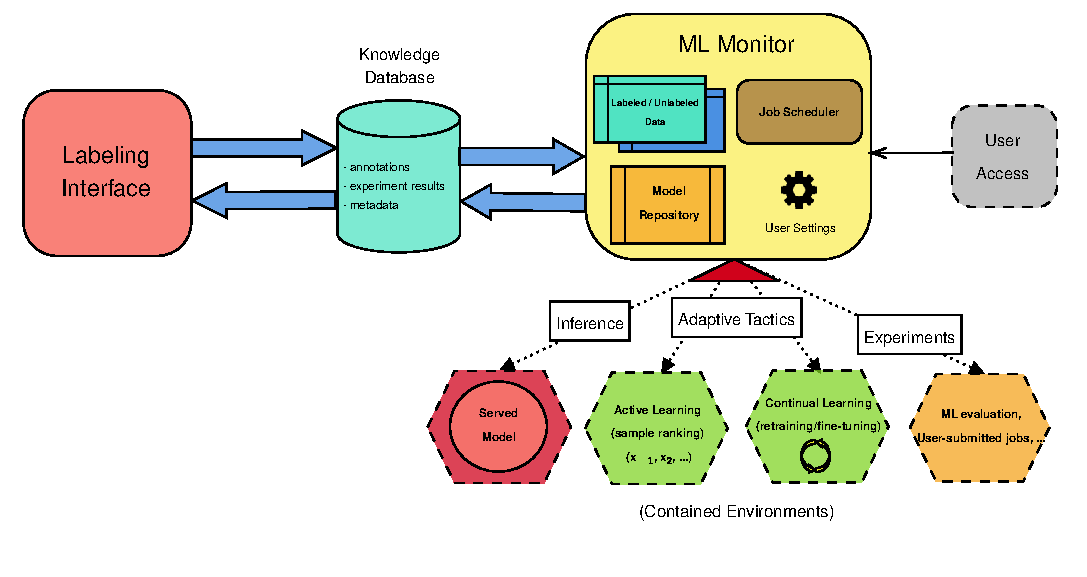
\includegraphics{ml-system-proposal.pdf}
        }
        \label{fig:system_proposal_diagram}
    \end{figure}

    
    
    \section{Components of the System} \label{sec:system_components}

    The system we propose in this work is comprised of five main components, which were explicitly designed to allow the implementation of adaptation tactics in a framework similar in fashion to MAPE-K loops (or at least inspired from it) and following the aspects described in section \ref{sec:design_aspects_considered}.
    
    
    \subsection{Knowledge Database} \label{sec:knowledge_db}

    The \textit{Knowledge Database}, which we denote as $\mathcal{K}$, is the source of truth of the system. It is the component that stores all the data and information that is relevant to the platform (the \textit{K} in MAPE-K). We have implemented it in our solution as a relational database (PostgreSQL) that stores all the data samples, annotations, and models that are part of the system.

    Thus as a relational database, $K$ can be characterized by the entities that comprise it and the relationships between them. Note we talk about `entities' as types of information that map to (have a relation with) other entities in the database. We also denote `object entities' as stored instances of these entities in $\mathcal{K}$.
    
    Throughout this chapter, we use the notation $entity_a \Rightarrow entity_b$ to denote a relationship between two entities in $K$, where $entity_b$ can be considered as an attribute of $entity_a$. For cases where the attribute of an entity is not another entity, but a value of some datatype, we use dot notation (e.g., for "$e.\texttt{name}$", \texttt{name} may be a string attribute of some entity $e$).

    With that in mind, we consider the following entities to be part of $\mathcal{K}$\footnote{ \nameref{appendix:db_er_diagram} shows the entity-relationship (ER) diagram of an implementation of the knowledge database (the one we use for our solution).}:

    \vspace{0.3cm}
    
    \begin{itemize}
        \item \textbf{Entity} $\boldsymbol{x \in \mathcal{K}}$ is a single \textit{data sample} that can be annotated by a human expert or by the system itself (e.g., a single clinical image, text, or a row in a table). Data samples have as attributes their corresponding annotations ($x \Rightarrow annotations$). We denote this entity $x$  because it is the information that can be used as input to an ML model - crucial to the processes of training and inference.
        \item \textbf{Entity} $\boldsymbol{annotation \in \mathcal{K}}$ is an \textit{annotation} of a data sample $x \in \mathcal{K}$ made by a human expert or by the system itself. Annotations have attributes related to their annotator ($annotation\Rightarrow annotator$), and the label of the annotation, which we characterize as a set of \textit{property} entities ($annotation\Rightarrow properties$). 
        \item \textbf{Entity} $\boldsymbol{p \in \mathcal{K}}$ is a property of a single $annotation$ object. Properties have as attributes their name and value ($p.\texttt{name}$, $p.\texttt{value}$), which we use to describe the information carried by that annotation. For example, a 'binary label' property may have values 1 or 0 depending on the annotation.
        \item \textbf{Entity} $\boldsymbol{annotator \in \mathcal{K}}$ is an entity that creates annotations  (and their corresponding properties) to any data sample $x$. It can be a human expert or an automated system. Annotators have a boolean $is\_automatic$ attribute ($annotator.\texttt{is\_automatic}$) that characterizes if the annotator is a model deployed to be used by the system (e.g., as part of an adaptation tactic or to make predictions on data). 
    \end{itemize}

    \vspace{-0.3cm}

    Figure \ref{fig:knowledge_db_schema} shows the entity-relationship (ER) diagram of the implementation of the knowledge database we designed for our solution. At the core of the schema are the same concepts that we listed above, we have only included a few more entities for data management purposes (e.g., \textit{project}, \textit{project\_annotator}, \textit{datastore} etc.) that are not very relevant to the design, so we won't discuss them in detail \footnote{For more details about the other entities in the implementation of the database, see \nameref{appendix:db_er_diagram}.}. 
    
    Note also that the \textit{artifact} entity in that diagram is equivalent to the \textit{x} entity we described above. For our use-case, these artifacts point to the location of the image files that we can use as input to our TB detection models, and the \textit{annotations} of these artifacts, along with their \textit{properties}, contain the labels of each of those images.

    Such is our implementation of $\mathcal{K}$ in this project. But to keep things general, we will formalize further how we describe the relations in $\mathcal{K}$ and how to denote the act of extracting information from it.

    \begin{figure}[t]
        \centering
        \caption{Entity-Relationship (ER) Diagram of the Knowledge Database ($\mathcal{K}$)}
        \hspace*{-0.5cm}
        \resizebox*{1.1\columnwidth}{!}{
            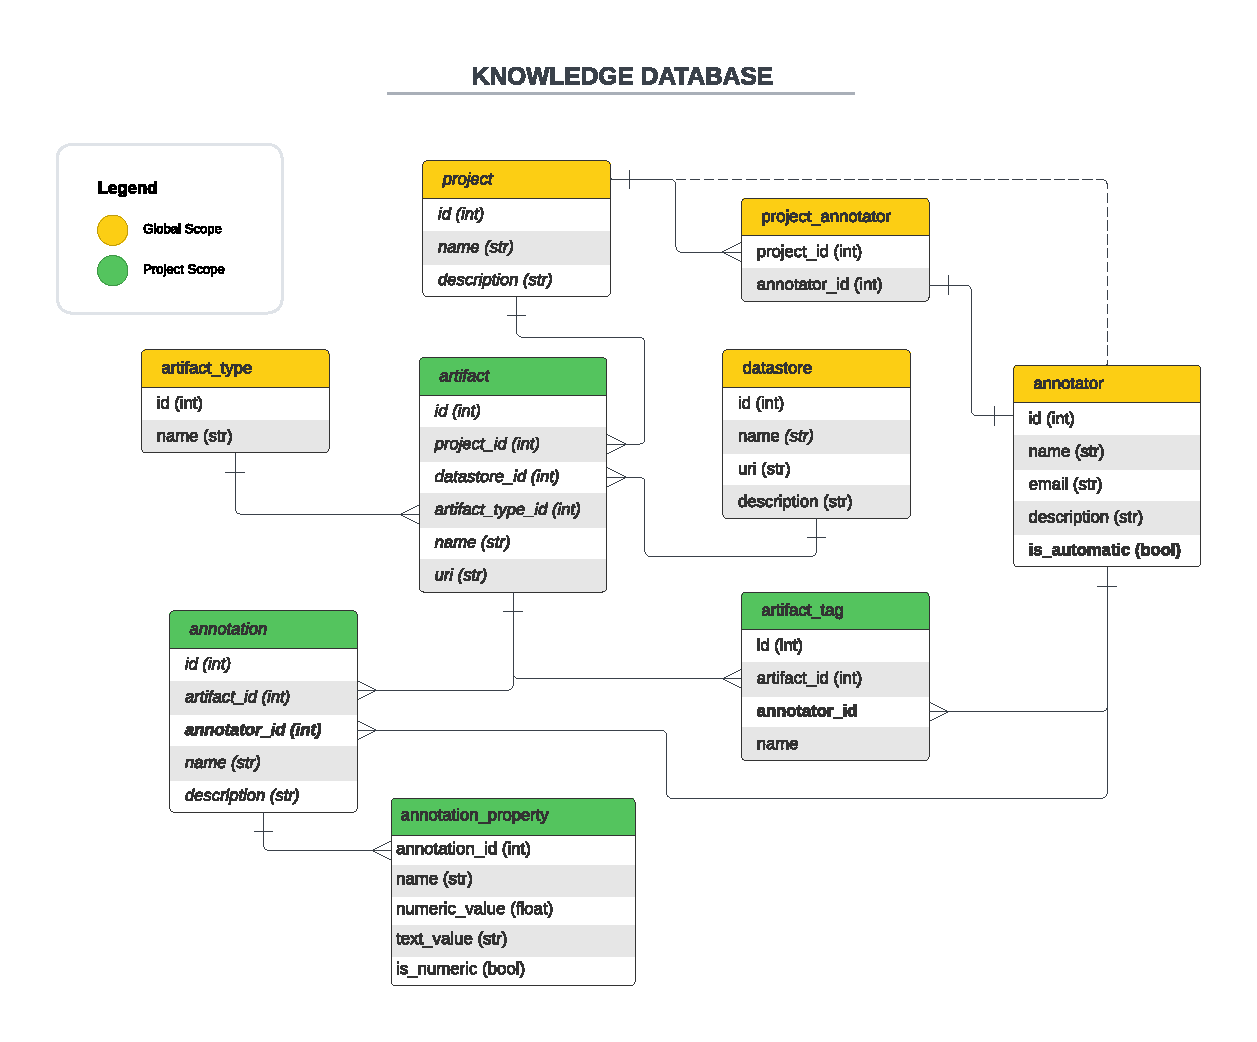
\includegraphics{knowledge_db_schema.pdf}
        }
        \label{fig:knowledge_db_schema}
    \end{figure}

    
    First of all, we note that a single data sample can have multiple annotations. We consider relationships like $\{x \Rightarrow annotations\}$ to denote a one-to-many mapping that returns all \textit{annotation} objects related to $x$. Similarly, we do the same with $\{annotation \Rightarrow properties\}$, and $\{annotator \Rightarrow annotations\}$. 
    
    Note we surround these types of relationships with curly brackets to emphasize that they return sets of entity objects in $\mathcal{K}$ (as opposed to single entity objects).

    In an abuse of notation, we also allow the use of $\Rightarrow$ for these sets of entities. For example, the expression $\{x \Rightarrow annotations \Rightarrow properties \Rightarrow property.\text{name}\}$ denotes the set of all names of the properties of annotations of $x$. This will be useful at the time of defining the algorithms for the tactics we'll formalize later in this chapter.

    \vspace{0.5cm}

    Furthermore, as a database, $\mathcal{K}$ can be queried to extract any information in it (be it as entity objects or attribute values). We will use the syntax described above, along with general relational algebra syntax\footnote{See: \href{https://en.wikipedia.org/wiki/Relational_algebra}{wikipedia.org/wiki/relational\_algebra}} \cite{silberschatzDatabaseSystemConcepts2011}, to denote that action.

    For example, to represent a query that gets all annotations in $\mathcal{K}$ that has a property named `label', we use the syntax:

    \vspace{-0.35cm}

    \[\{a \in \mathcal{K}_{annotation} \mid \text{`label'} \in \{a \Rightarrow properties \Rightarrow property.name\}\}\]

    \vspace{-0.2cm}

    Where $\mathcal{K}_{annotation}\subset\mathcal{K}$ is the set of all $annotation$ object entities in the database (we'll use the same notation to express sets of all objects of a single entity when convenient  \footnote{In \nameref{appendix:db_er_diagram}, we include an example of how this query might look like in standard SQL syntax.}.  

    % We also assume that when a single entity object is added to $\mathcal{K}$, it is assigned a unique identifier that can be used to reference it, which is a standard practice in database design.  

    % \vspace{-0.3cm}
    \subsection{Model Repository}
    % \vspace{-0.2cm}

    As mentioned in section \ref{sec:design_aspects_considered}, we consider the \textit{model repository} to be the `bag' of models available to the system. We denote it as $\mathcal{M}$, and a single model as $m \in \mathcal{M}$.
    
    $\mathcal{M}$ stores the models that are currently deployed in the system and are being actively monitored to be continuously adapted. Thus, it can be seen as a subset of all models that have been trained and evaluated (since some of them may have been discarded or replaced at some point).
    
    The action of adding a model to $\mathcal{M}$ we denote as $m \rightarrow \mathcal{M}$, and the action of removing a model from $\mathcal{M}$ as $m \leftarrow \mathcal{M}$. Consequently, we can consider that the action of updating a model in $\mathcal{M}$ is the combination of both actions, with $m_{new}$ being added and $m$ removed.

    Any $m \in \mathcal{M}$ can be seen as a function that takes a data sample $x \in \mathcal{K}$ as input and outputs a prediction $\hat{y}$, which can be used and tracked by the system. We denote this function as $m(x) = \hat{y}$ (for $x \in \mathcal{K}$).

    One aspect of the design of the system is that we assume a one-to-one correspondence between models in $\mathcal{M}$ and the automatic annotators in the knowledge database $\mathcal{K}$. Thus, sometimes we treat them as equivalent entities in our design of the framework.
    
    That is, we make the following equivalence:
    
    \vspace{-0.5cm}

    \[
        \begin{gathered}
        \text{For: }\ \  \mathcal{K}_{\mathcal{M}} =  \{\textit{annotator} \in \mathcal{K} \mid \textit{annotator} \Rightarrow \text{ is automatic}\} \\ 
        m \in \mathcal{M} \iff m \in \mathcal{K}_{\mathcal{M}}
        \end{gathered}
    \]
    
    From an implementation perspective, the mapping between the model repository and the knowledge database could be done by using the same identifier for both entities (which is what we do in our implementation), then, when you query a model from $\mathcal{M}$, you can also query its corresponding \textit{annotator} entity from $\mathcal{K}$.
    
    Thus, from this point on, we will use $m$ to refer to both a model in the model repository and an automatic annotator in the knowledge database interchangeably. We also assume that any process that can pull $m$ from $\mathcal{M}$ can also do it from $\mathcal{K}_\mathcal{M}$ and use it with the same function without any distinction, which will be useful for the design of the adaptation tactics that we'll describe in the next section.

    Furthermore, we assume that either $M$ or $K$ can track the samples $x \in \mathcal{K}$ that are associated with $m$ (the samples that can be used as input to $m$). We denote this set of samples as $\mathcal{K}_m$. This feature could be implemented by adding attributes or entities to the database that map ML models to data samples but to simplify things we'll refer to it simply stating it as the set $\{x \in \mathcal{K} \mid x \text{ is associated with } m\}$ (for some $m \in \mathcal{M}$).

    \vspace{-0.3cm}
    \subsection{ML Monitor} \label{sec:ml_monitor}

    The ML monitor is how we refer to the component that is in charge of deploying the models in $\mathcal{M}$ in a production and/or experimental environment and continuously monitoring their performance on the data samples in $\mathcal{K}_m$.

    Alongside the Knowledge database and job scheduler, the functionalities of the ML monitor complement our implementation of the MAPE-K loop that we propose in this work. We consider it to be the component that is in charge of the \textit{monitoring}, \textit{analysis}, and \textit{planning} phases of the loop (MAP), while the job scheduler (which we describe in \ref{sec:job_scheduler}), the \textit{execution} phase.

    Thus the job of the ML monitor is to keep track of all models in $M$, continually analyze how they perform when new data arrives and decide which strategy to take. Note that in figure \ref{fig:system_proposal_diagram}, we've depicted the model repository inside this component to emphasize the fact that only ML models in $\mathcal{M}$ are being monitored by the system. 
    
    We formalize the idea of monitoring and analyzing the performance of ML models by introducing the concept of \textit{benchmarks}, functions $B(m, \mathcal{K}_m)$ that take a model $m \in \mathcal{M}$ and some data associated with it and outputs a metric of how well it performs.
    
    The benchmark function can be any metric that is relevant to the stakeholders of the application as long as it works for the model and data (i.e., no need to assess binary classification performance on clustering tasks). 
    
    Since we consider that model and its relevant benchmarks are strictly associated, we assume that the platform can query the benchmark functions associated with any model. We denote this set $B_m$ for some $m \in \mathcal{M}$. We implement this in our system as configuration settings that users can manually pass to the ML monitor directly (see Figure \ref{fig:system_proposal_diagram}).
    
    For example, in the case of TB detection with the models we have developed for this work, we can use metrics like the \textit{accuracy} or \textit{F1-score} of the model on the image samples. When new microscopy images are available, the system may launch tasks that prioritize the annotation of certain samples (active learning) to then benchmark the performance of the model compared to the true annotations and launch an adaptive active if it drops below a threshold.

    % The idea is that the ML monitor can use this benchmark function to keep track of the performance of the models in $\mathcal{M}$ and use that to trigger adaptation tactics (that are launched by the job scheduler). For example, if the benchmark function returns a value that is below a certain threshold, the ML monitor can trigger an adaptation tactic to try to improve the performance of the model.

    
    % Therefore, the benchmark function defines the criteria used by the system to launch an adaptation tactic. We

    Because this process is fully data-driven (we only need to select which samples to pass to the already deployed model), it can be easily automated and be done without any human intervention. 
    
    % However, the ML monitor can also be used to inform the stakeholders of the application about the performance of the models in $\mathcal{M}$, and these can in turn use that information to make decisions about the future of the application or the design of new benchmarks and tactics that try to improve the models on any relevant metric.


    \vspace{-0.6cm}
    
    \subsection{Job Scheduler} \label{sec:job_scheduler} \todo{separate ML monitor from job scheduler in the diagram}
    % \vspace{-0.3cm}

    The job scheduler is the component that is in charge of actually launching the adaptation tactics that are part of the system. We denote it as $\mathcal{J}$, and a single job as $j \in \mathcal{J}$. 

    We consider $j$ to be any function that requires the use of the models in $\mathcal{M}$. Which in our case can range from running a benchmark test, evaluating the performance/efficacy of models, and initiating adaptation tactics.

    The operations of the job scheduler are primarily governed by the benchmark outcomes relayed from the ML monitor. If the benchmark performance of a model is flagged as underperforming (i.e., below a certain threshold), the ML monitor will interact with $J$ to trigger an adaptation tactic on that specific model.

    Furthermore, we consider $j$ to be any function that requires the use of the models in $\mathcal{M}$. This includes any benchmark, model evaluations, and adaptation tactics.
    
     From a practical point of view, having a job scheduler allows us to centralize the execution of all operations relating to the models in $\mathcal{M}$. This design choice reduces the overall complexity of the system and simplifies the management of the ML models (for example, only $J$ needs access to their actual raw files).

     Another point that we made sure of in the design of this component is to require each task/job to be independent of each other and containerized in its own computing environment so that they can be executed in parallel, or even put in a distributed computing setting. Which may allows to scale system like this to handle many models and data.
    

   \subsection{Labeling Interface} \label{sec:labeling_interface}

   The final component we discuss in this section is the \textit{labeling interface}. The idea of this component comes directly from the objective that a system like the one proposed should ease annotation efforts to optimize the costs associated with them.  

   The main aspect of this component is that it allows a human expert to annotate data samples in $\mathcal{K}$ and add them to the knowledge database, bringing them closer to the adaptation process.
   This human-in-the-loop approach can then be used to inform the next steps of the adaptation process.   
   
   Unlike the other components, we make no formalization about how the labeling interface should work, we consider that to fully depend on the kind of tasks that are being solved by the ML models and the data that is being annotated. 
   
   Thus, the design of such an interface should be oriented towards enabling - promoting even - these types of interactions, as to consider the information gained from them for the development of adaptation tactics that target the models monitored by the platform. 
   
   For the project in this work, we implement this interface to facilitate the identification of TB bacilli in sputum-smear microscopy images. The interface was designed to show these kinds of images (pulled dynamically from the database) along with the bounding boxes (rectangular regions in the image) where a bacillus was identified.

   Figure \ref{fig:labeling_interface} shows the interface that we developed for this project.

   \begin{figure}
       \centering
       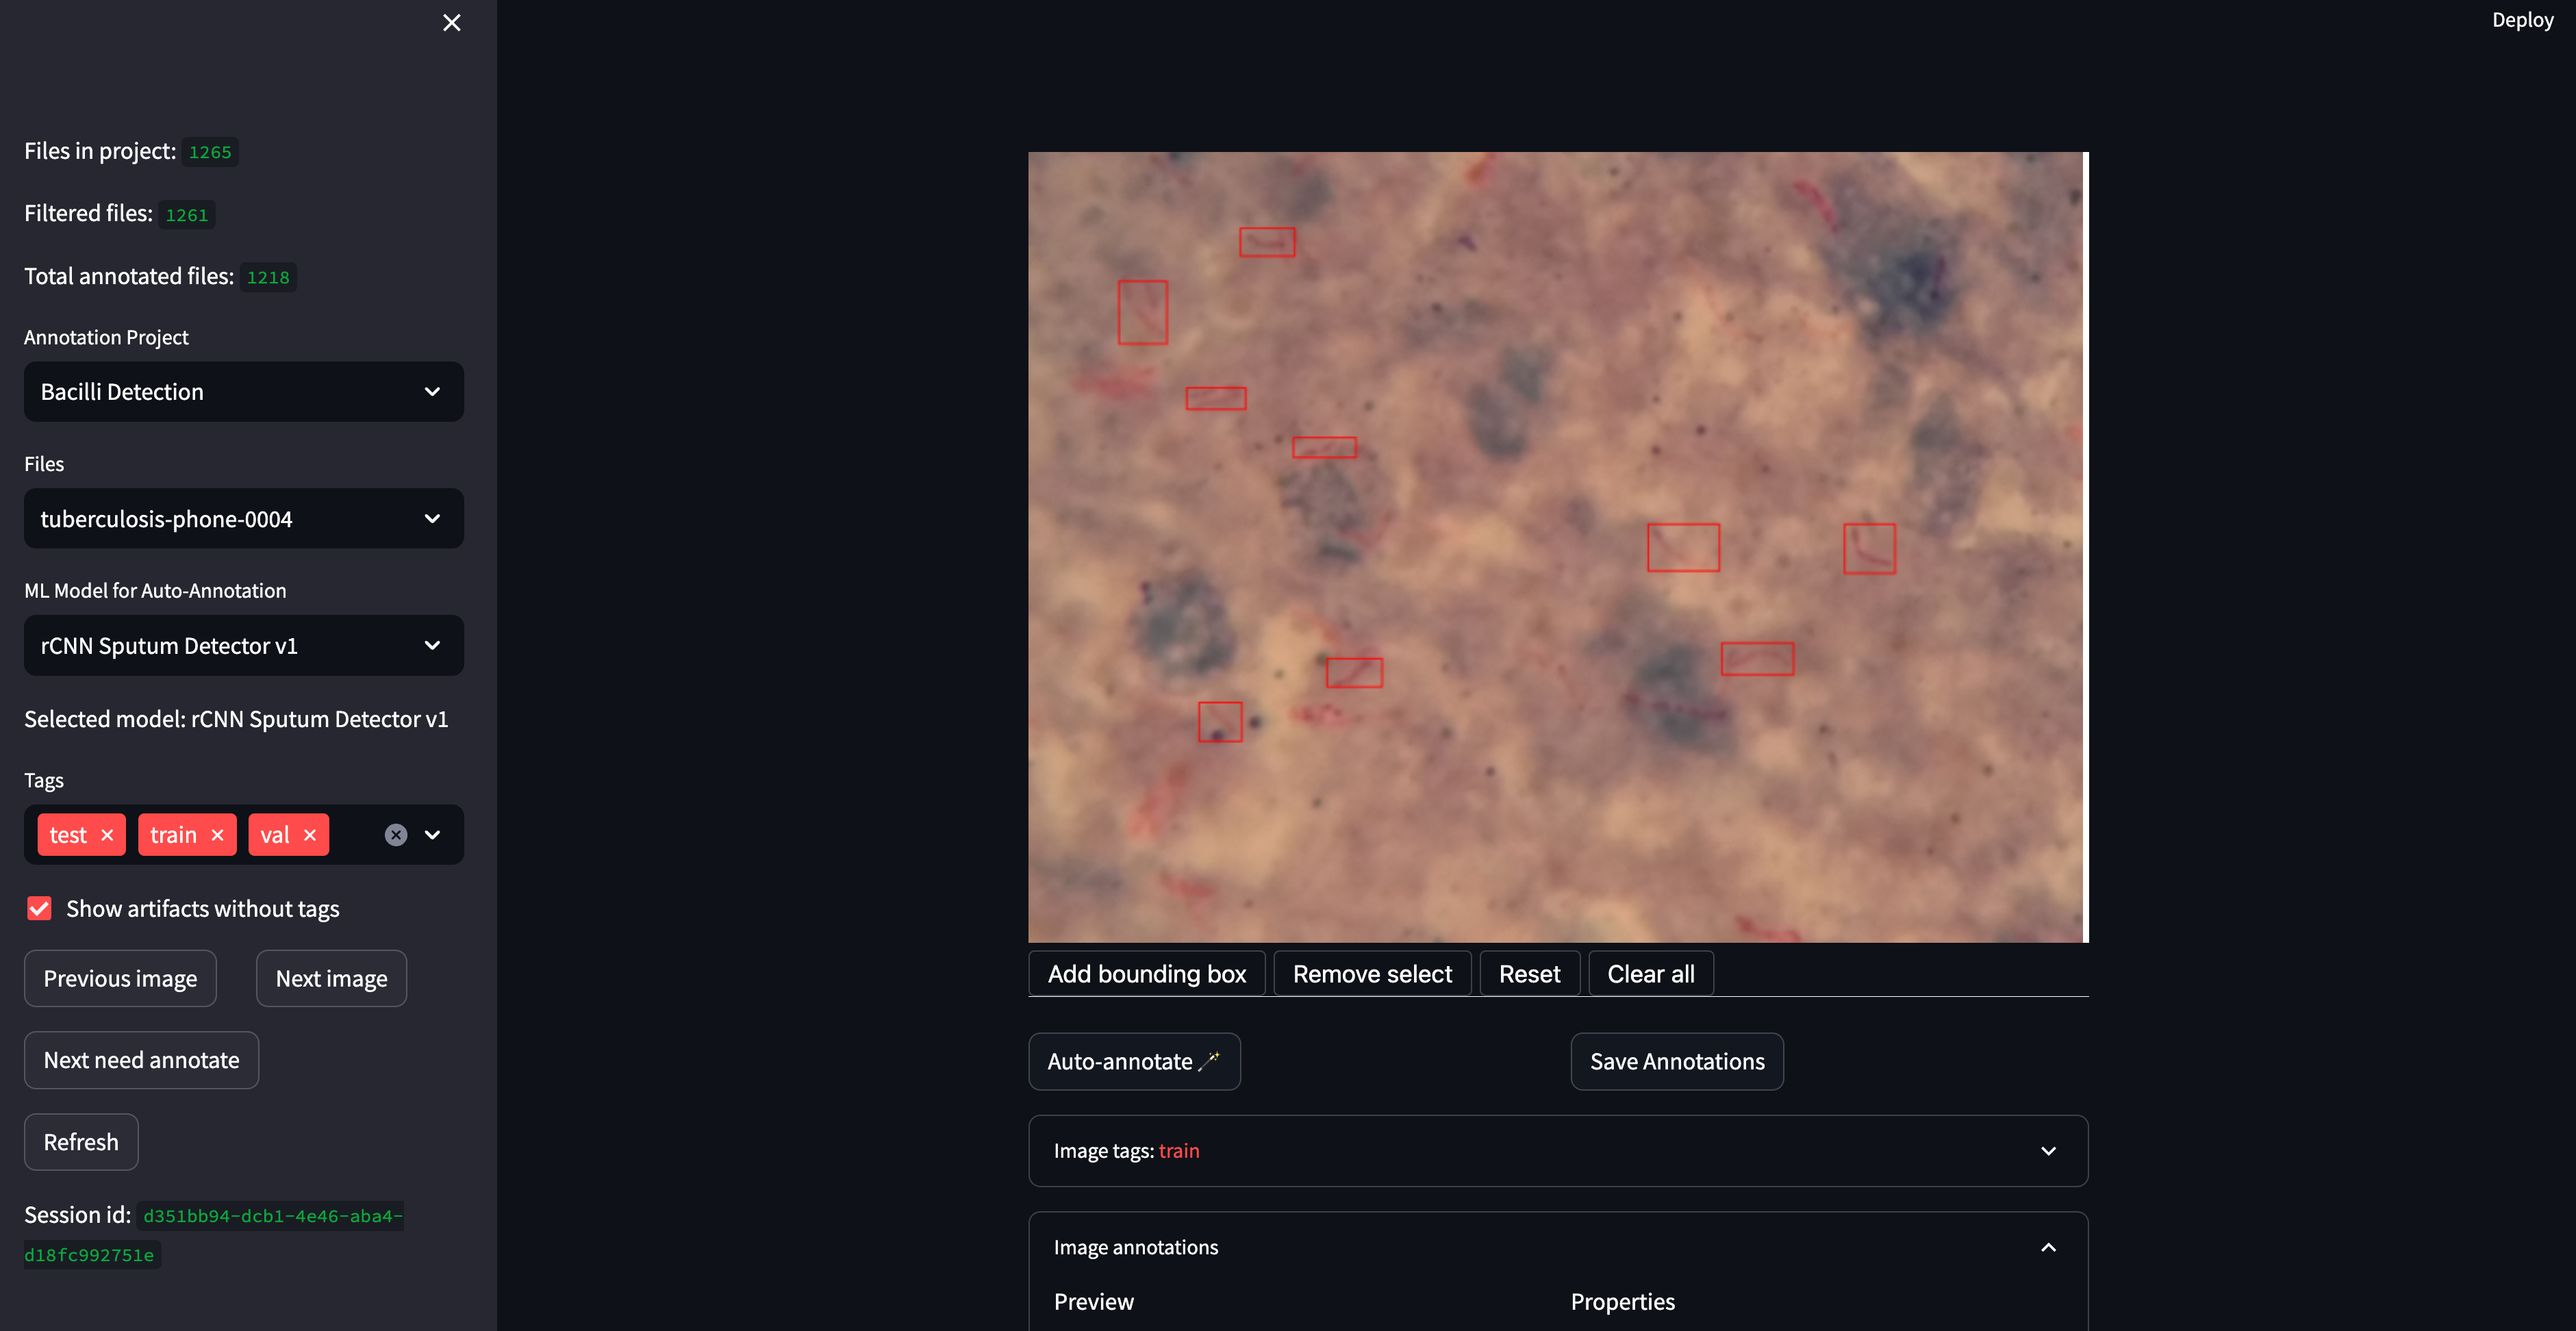
\includegraphics[width=1\linewidth]{figures/annotation_platform_capture.png}
       \caption{Labeling Interface to annotate TB Bacillus:\\\footnotesize The interface includes buttons to filter through the relevant samples in the database, and add boxes in regions of the image where the bacilli is identified. Annotations are then sent to the database to be compared with model predictions, which may trigger an adaptation tactic.}
       \label{fig:labeling_interface}
   \end{figure}

   The interface also allows annotators to create their own bounding boxes in the regions of the image where they identify bacilli are located and compare that with the predictions of the model. This information is recorded and the annotations and relevant properties are saved to the knowledge database.

   Adaptation tactics like \textit{active learning} can then take the new annotations to update their prior beliefs about the samples that are most important to annotate and with that improve the productivity of the entire process.


    \section{Formalizing the Adaptive Process} \label{sec:formalizing_adaptive_process}


    We follow this section formalizing some of the adaptation tactics we consider could be applied to the system we propose. These tactics are the main drivers of the adaptation process, and thus, we consider them to be the platform's most critical components.

    Thus, to provide a general understanding of how these tactics work and interact with the ideas we have described in this chapter, we will write down the algorithms that fully describe them, along with a brief explanation of how they work and their purpose within the context of this project.

    
    
    \subsection{Continual Learning}
    \vspace{-0.45cm}
    
    We use continual learning as a base for the adaptation tactics we propose. The main idea of a continual learning process based on the aspects of our system is to use the data available in the knowledge database to train ML models that can be used to replace the ones that are currently deployed. 
    
    The way this is approached is by training a new model, $m_{new}$ with the data available in the knowledge database and then comparing its performance with the $m$ that is currently deployed. If $m_{new}$ outperforms $m$ in the relevant metrics, then it is deployed in its place. Otherwise, the old model is kept, and the process is repeated in the future.

     % aqui creo que te olvidaste de presentar el fine-tuning
    Furthermore, we can consider two different approaches to the continual learning process: We can either \textit{retrain} the model, $m$ or fine-tune it. We characterize the two approaches based simply on the data taken into account during the training process. 
    
    In the case of retraining, the model is trained with all the data available in the knowledge database that is associated with it, while in the case of fine-tuning, the model is trained with the new data only (as with transfer learning). In the latter case, the already trained model is used as a starting point, and its parameters are updated with the new data.
    
    
    The following pseudocode describes the continual learning process:

    \vspace{0.25cm}

    \begin{algorithm}[H]
        \SetAlgoLined 
        \KwIn{model $m \in \mathcal{M}$, data $\mathcal{K}_m' \subset \mathcal{K}_m $}
        \KwResult{\texttt{success} if $m_{new} \in \mathcal{M}$, \texttt{failure} otherwise}
        \textbf{Let} $m_{new} = \texttt{Train}(m, \mathcal{K}_m)$ \\
        \emph{The platform should be able to complete the training process of $m_{new}$} \\
        \For{$B_i \in \{m\Rightarrow B_m\}$}{
            \emph{$B_m$ is the set of benchmark functions associated with $m$} \\
            \If{$B_i(m_{new}, \mathcal{K}_m')$ better than $B_i(m, \mathcal{K}_m')$}{
                \emph{The new model outperforms the old one} \\
                $m \leftarrow \mathcal{M}$ \\
                $m_{new} \rightarrow \mathcal{M}$ \\
                \Return \texttt{success}
            }
        }
        \Return \texttt{failure}
        \caption{ContinualLearning($m$, $\mathcal{K}_m'$)}
        \label{alg:continual_learning}
    \end{algorithm}

    % And to illustrate the idea that the continual learning process serves as a base for the other adaptation tactics, we can define transfer learning as a special case of continual learning where the model is fine-tuned with a subset of data that wasn't used to train it:
    
    % \vspace{0.3cm}
    % \begin{algorithm}[H]
    %     \SetAlgoLined 
    %     \KwIn{model $m \in \mathcal{M}$, data $\mathcal{K}_m' \subset \mathcal{K}_m $}
    %     \KwResult{$m_{new} \in \mathcal{M}$, a new model adapted from $m$}
    %     \textbf{Let} $m_{new} = \texttt{FineTune}(m, \mathcal{K}_m)$ \\
    %     \emph{The platform should be able to complete the fine-tuning process of $m_{new}$} \\
        
    %     \caption{TransferLearning($m$, $\mathcal{K}_m'$)}
    %     \label{alg:transfer_learning}
    % \end{algorithm}
    
    % \begin{algorithm}[H]
    %     \SetAlgoLined % requires \usepackage{algorithmic}, or use algorithmicx
    %     \KwResult{Annotated data} % requires \usepackage{algorithmic}
    %     \While{not enough annotated data}{
    %         \For{each model $m_i \in \mathcal{M}$}{
    %             \For{each data point $x \in \mathcal{K}$}{
    %                 \If{$x$ is relevant to $m_i$}{
    %                     annotate $x$
    %                 }
    %             }
    %         }
    %     }
    %     \caption{ContinualLearning}
    %     \label{alg:continual_learning}
    % \end{algorithm}

    \subsection{Active Learning}

    We consider the problem of active learning as a way to reduce the amount of data that needs to be annotated by a human expert. In an active learning setting, we assume that there's a way to rank the data based on their relevance to the training of a given model. 
    
    Thus, we can use this ranking to select the data that should be annotated to optimally train the model in a continual learning process. We use this idea to present a general approach to active learning as an adaptation tactic in the context of the system we propose and formalize it as follows:

    Let $R(m, \mathcal{K}_s)$ be a ranking function that \textbf{ranks the samples associated with a model}. $R(m, \mathcal{K}_s)$ takes a model $m\in\mathcal{M}$ and a set of samples $\mathcal{K}_m \subset \mathcal{K}$ of data associated with $m$ and returns an \textbf{ordered set}  of the samples in $\mathcal{K}_m$, ranked according to their `importance' (however that is defined) to the training of $m$. 
    % Thus, we can consider $R$ to be a model-specific adaptation tactic.

    The pseudocode below describes the process of ranking the data in $\mathcal{K}_m$ with $R$. The ranking is stored in $\mathcal{K}_m$ as annotations of the data made by $m$ itself rather than a person (note that here we `annotate' the samples with the ranking value, not the actual label).
    
    % \KwResult{A ranking of the data in $\mathcal{K}_m$ based on their importance to the training of $m$}

    % sample ranking is the algorithm applied by R to rank the data in $\mathcal{K}_m$.
    \vspace{0.2cm}
    \begin{algorithm}[H]
        \SetAlgoLined
        \KwIn{ranking function $R$, model $m$ in $\mathcal{M}$, pool of data samples $\mathcal{K}_p \subset \mathcal{K}$}
        % apply the R function to rank the data in $\mathcal{K}_m$ \\
        \textbf{Let} $\mathcal{K}_{ranked} = (x_1, x_2, \dots, x_n) = R(m, \mathcal{K}_s)$ \\
        \emph{Note $\mathcal{K}_{ranked}$ contains the same samples as $\mathcal{K}_p$ but ordered based on their `importance' to the training of $m$} \\
        % we now add annotations to the data in $\mathcal{K}_{s}'$ \\
        \For{$i \in \{1, \dots, n\}$}{
            $x = \mathcal{K}_{ranked}'[i]$ \\
            \emph{The statements below are meant to depict direct modifications to $\mathcal{K}$} \\
            $a_i$ = \textbf{new} $annotation(annotator = m)$ \\
            $p_i$ = \textbf{new} $property(name = \text{`ranking'}, value = i)$ \\
            $a_i \Rightarrow properties = \{p_i\}$ \\
            $x \Rightarrow annotations = \{a_i\} \cup (x \Rightarrow annotations)$ \\
            \emph{Note that this creates new object entities $a_i,p_i \in \mathcal{K}$} 
        }
        \caption{ImportanceSampling($R$, $m$, $\mathcal{K}_p$)}
        \label{alg:sample_ranking}
    \end{algorithm}

    \clearpage

    % We can then use importance sampling to select the data that should be annotated to optimally train $m$ in a continual learning process.
    
    Importance sampling allows the platform to prioritize the labeling of the samples that are most optimal to the learning process (i.e., the labeling interface can show the annotators the important samples so that they are labeled before any other in $K_m$). Then, with every new (important) sample we label, we can proceed with continual learning on the newly annotated data and repeat this process until there is no more data to annotate.

    This is the concept behind active learning, which we formalize in the algorithm below:

    \begin{algorithm}[H]
        \SetAlgoLined
        \KwIn{ranking function $R$, model $m \in \mathcal{M}$, knowledge database $\mathcal{K}$}
        \textbf{Let} 
        % query the samples ranked by $m$ that are 'ranking' \\
        $\mathcal{K}_{ranked}$ = $\{x \in \mathcal{K} \mid (\text{`ranking' } \in (x \Rightarrow annotations \Rightarrow properties \Rightarrow property.name)) \land ((x \Rightarrow annotations \Rightarrow annotator) = m)  \}$ \\
        \emph{Note $\mathcal{K}_{ranked}$ is the set of samples in $\mathcal{K}$ that have been ranked before for $m$} \\
        \If {$K_{ranked} = \emptyset$}{
            \emph{We rank the samples associated with $m$} \\
            $\boldsymbol{\mathcal{K}_s} = \{x\in \mathcal{K}_m \mid 
            \{a \in \{x \Rightarrow annotations\} \mid (a \Rightarrow annotator) \notin \mathcal{M} \} = \emptyset\}$ \\
            \emph{Note $\mathcal{K}_s$ is the set of samples that are relevant to $m$ and are not yet annotated by a human} \\
            \If{$\mathcal{K}_s = \emptyset$}{
                \emph{There's no data to annotate} \\
                \textbf{exit} \\
            }
            \emph{Rank the samples in $\mathcal{K}_s$ and start over} \\
            \texttt{ImportanceSampling}($R$, $m$, $\mathcal{K}_s$) \\
            \Return \texttt{ActiveLearning}($R$, $m$,  $\mathcal{K}$) \\
        }
        $\mathcal{K}_{ranked}^+ = \emptyset$ \\
        % \emph{$\mathcal{K}^+$ will collect all the samples that have been annotated} \\
        \For{$(x_i, \dots x_n) \in \mathcal{K}_{ranked}$}{
            \emph{Note we assume the samples in $\mathcal{K}_{ranked}'$ are sorted by their `ranking' value} \\
            \textbf{annotate} $x_i$ \\
            $\mathcal{K}_{ranked}^+ = \mathcal{K}_{ranked}^+ \cup \{x_i\}$ \\
            \If{\texttt{ContinualLearning}(m, $\mathcal{K}_{ranked}^+$) $ = $ \texttt{success}}{
                \emph{start over}\\
                \Return \texttt{ActiveLearning}($R$, $m$,  $\mathcal{K}$) \\
            }
        }
        \caption{ActiveLearning ($R$, $m$, $\mathcal{K}$)}
        \label{alg:active_learning}
    \end{algorithm}

    Note we assume that with the \textbf{annotate} command, we assume that the annotation is done by a human that has domain knowledge about the data in $\mathcal{K}_m$. Thus, a delay between one iteration and the next of the \textbf{while} loop shown in the algorithm above is expected. 

    \subsection{Other adaptive processes}

    We only implement experiments with the two adaptation tactics described above, but we can show that the system we propose can be extended to include other tactics by simply being selective on the benchmark functions and relevant data that we pass to the continual learning tactic, just as we did with active learning.

    For example, to implement adversarial training as an adaptation tactic in this system, we can define a benchmark function that measures the robustness of the model to adversarial attacks (i.e. letting $B(m, \mathcal{K}_m)$ be a function that returns the accuracy of $m$ on adversarial samples). 
    
    Then, we can pass to the continual learning process data samples that are adversarial to the model (which can be priorly tagged by annotators as such). Thus the whole process of adversarial training reduces to $\texttt{ContinualLearning}(m, \mathcal{K}_{adv})$ where $\mathcal{K}_{adv}$ is a set of adversarial samples to train $m$ with (that are available in the knowledge database).

    Furthermore, Knowledge distillation can be formalized by letting the training function \texttt{Train($m, \mathcal{K}_m$)} be a distillation process that uses the predictions of the current model $m$ as a soft target for a smaller $m_{new}$. We can then use a benchmark function $B(m_{new}, \mathcal{K}_m)$ of how close the predictions of $m_{new}$ are to those of the previous $m$.
        
  %% añade en algun sitio las imagenes que has usado para los experimentos, aunque has mencionado que vas a usar la misma que yo aclara el número que ass usado en cada etapa, si las preprocesaste
% \printbibliography
\end{document}